% Communications Physics version (Article): Introduction / Results / Discussion / Methods.
% Main text (Introduction, Results, Discussion) is kept below ~5000 words; all proofs are in Methods.
\documentclass[11pt]{article}

\usepackage[a4paper,margin=2.5cm]{geometry}
\usepackage{amsmath,amssymb,amsthm,bm}
\usepackage{mathtools}
\usepackage{graphicx}
\usepackage{xcolor}
\usepackage{authblk}
\usepackage[super,sort&compress,comma]{natbib}
\usepackage{setspace}
\usepackage[running]{lineno}
\usepackage[colorlinks=true,linkcolor=blue!60!black,citecolor=blue!60!black,urlcolor=blue!60!black]{hyperref}

\graphicspath{{figures/}}
\onehalfspacing
\linenumbers

% ---------------------------------------------------------------------------
% Theorem environments and macros
% ---------------------------------------------------------------------------
\newtheorem{theorem}{Theorem}
\newtheorem{proposition}{Proposition}
\newtheorem{lemma}{Lemma}
\newtheorem{corollary}{Corollary}
\theoremstyle{definition}
\newtheorem{definition}{Definition}

\newcommand{\tr}{\operatorname{tr}}
\DeclareMathOperator{\artanh}{artanh}
\newcommand{\vecr}{\vec r}
\newcommand{\mhat}{\hat m}
\newcommand{\nhat}{\hat n}
\newcommand{\vsigma}{\vec\sigma}
\newcommand{\maj}{\prec}
\newcommand{\omplus}{\omega_{\oplus}}
\newcommand{\omtimes}{\omega_{\otimes}}
\newcommand{\sqc}{\sqrt{c}}
\newcommand{\todo}[1]{\textcolor{red}{[TODO: #1]}}

\title{Majorization uncertainty bounds for incompatible binary measurements cannot be saturated}

\author[1,2,3]{Rui Zhu}
\author[4]{Gilad Gour}
\author[1,2,3,*]{Marcelo F. Ciappina}
\affil[1]{Department of Physics, Guangdong Technion-Israel Institute of Technology, Shantou 515063, China}
\affil[2]{Technion--Israel Institute of Technology, Haifa 32000, Israel}
\affil[3]{Guangdong Provincial Key Laboratory of Materials and Technologies for Energy Conversion, Guangdong Technion-Israel Institute of Technology, Shantou 515063, China}
\affil[4]{\todo{affiliation(s) to be provided by Gilad}}
\affil[*]{Corresponding author: marcelo.ciappina@gtiit.edu.cn \todo{confirm corresponding author}}
\date{}

\begin{document}
\maketitle

% ---------------------------------------------------------------------------
\begin{abstract}
\noindent
Majorization turns the uncertainty principle into a single state-independent
probability vector that bounds every Schur-concave measure of uncertainty at
once. We determine what this universality costs for two binary measurements.
We prove that the optimal majorization vectors are attained by no state unless
the measurements commute, so every bound they imply for a strictly
Schur-concave measure, including the Shannon entropy, is strict; only the
R\'enyi entropies of order zero and infinity are bounded tightly. For two qubit
bases the direct-sum Shannon bound falls up to 22\% short of the exact minimum,
yet beats the Maassen--Uffink relation unless the bases are nearly mutually
unbiased. We obtain the optimal bound for noisy and biased measurements in
closed form and in any finite dimension, and show that detector bias, unlike
detector noise, can invalidate ideal-detector uncertainty relations and the
steering tests built on them; a single inequality decides when this happens.
\end{abstract}

% ===========================================================================
\section*{Introduction}
% ===========================================================================

The uncertainty principle is one of the defining features of quantum
mechanics\cite{Heisenberg1927,Robertson1929,BuschHeinonenLahti2007}: some pairs
of measurements cannot both have predictable outcomes, however carefully the
system is prepared. This preparation uncertainty, distinct from the
measurement uncertainty that limits joint measurements\cite{BuschLahtiWerner2014},
has become a quantitative resource. It underlies the security of quantum key
distribution\cite{BB84,Berta2010,TomamichelRenner2011}, gives experimentally
accessible criteria for entanglement\cite{HofmannTakeuchi2003,Guhne2004,Berta2010}
and for Einstein--Podolsky--Rosen steering\cite{Walborn2011,Schneeloch2013,Uola2020},
and is closely related to the incompatibility of
measurements\cite{HMZ2016,Guhne2023}. These applications need relations for
measurements with finitely many outcomes whose bounds do not depend on the
state. Robertson's variance relation\cite{Robertson1929} does not provide them;
entropies of the outcome distributions
do\cite{Hirschman1957,Beckner1975,BBM1975,Deutsch1983,Kraus1987}, the best known
example being the Maassen--Uffink (MU) relation\cite{MaassenUffink1988}, and
entropic uncertainty relations are now a broad field with many applications
and experimental tests\cite{WehnerWinter2010,Coles2017,deVicente2008,ColesPiani2014,Prevedel2011,LiXu2011}.

Each entropic relation, however, constrains a single measure of uncertainty,
whereas different tasks call for different measures: the Shannon entropy
quantifies average information, the min-entropy governs guessing
probabilities\cite{KRS2009}, and the R\'enyi and Tsallis families interpolate
between these and other extremes. Majorization\cite{MarshallOlkin2011}, the
order that captures when one distribution is more disordered than another and
a central tool of quantum information
theory\cite{Nielsen1999,Gour2015,ChitambarGour2019}, treats all of them at once.
One seeks a single state-independent vector that majorizes the outcome
statistics of every state; every uncertainty measure that respects
majorization then inherits a bound from this one vector. The programme was
initiated by Partovi\cite{Partovi2011} and developed into universal uncertainty
relations by Friedland, Gheorghiu and Gour\cite{FGG2013} and by Pucha{\l}a,
Rudnicki and {\.Z}yczkowski\cite{PRZ2013}; Rudnicki \emph{et al.} introduced the
stronger direct-sum form\cite{RPZ2014}. Majorization uncertainty relations have
since been extended to generalized measurements, mixed states and quantum
operations\cite{RasteginZyczkowski2016,Baek2019,Puchala2018}, made optimal in the
majorization lattice\cite{Li2016,LiQiao2019,Yuan2023}, tested
experimentally\cite{Wang2020,Yuan2023} and turned into steering
witnesses\cite{YangQiao2026}.

What does this universality cost? Partovi already remarked that the optimal
majorization vector is in general not the statistics of any state, so that a
``minimum-uncertainty state'' need not exist in this framework\cite{Partovi2011};
the point was recently reiterated in a review\cite{Conlon2026}. Li and Qiao
observed that the partial sums of the optimal qubit bound are usually reached by
different states, and that its Shannon entropy falls short of the optimal
Shannon bound in examples\cite{LiQiao2018}. What has been missing, even in the
simplest setting, is a proof of when the optimal bounds are attained, an account
of what non-attainment implies measure by measure, and an understanding of how
the bounds behave for the imperfect measurements performed in experiments.

Here we give this account for two binary (two-outcome) measurements, a setting
in which every step can be carried out in closed form. Unless the measurements
commute, no state attains either optimal majorization vector, so every bound it
implies for a strictly Schur-concave measure is strict; only the R\'enyi orders
zero and infinity are bounded tightly. The cost is substantial: for two qubit
bases the direct-sum Shannon bound falls short of the exact minimum by up to
22\%. Even so, it outperforms MU unless the measurement axes are within about
nine degrees of orthogonal, and its ratio to the exact minimum tends to one,
though only logarithmically, as the measurements approach compatibility. For
noisy and biased measurements we obtain the optimal direct-sum bound in closed
form, for qubits and in any finite dimension. This bound has an immediate
practical consequence. Detector noise can only increase uncertainty, so bounds
derived for ideal detectors remain valid, but detector bias---produced, for
instance, by mismatched detection efficiencies or by click/no-click
detection---can push the statistics of a state outside the ideal quantum set.
The single inequality $\Lambda\le2\sqrt c$, between a quantity of the measured
effects and the overlap of the ideal ones, decides whether the ideal relation
survives; when it fails, an uncertainty-based steering test can certify steering
for a product state.

Several ingredients are known, and we credit them where they are used: the
optimal bounds for two qubit bases are special cases of
Refs.~\citenum{PRZ2013,FGG2013,RPZ2014} and their optimality and saturating
states were found by Li and Qiao\cite{LiQiao2019}; the achievable expectation
values fill an ellipse\cite{LiQiao2015,KTW2014,Abbott2016}; the direct-sum bound
for unbiased unsharp qubit observables was evaluated by Baek
\emph{et al.}\cite{Baek2019}; and the relation between overlap and
anticommutator in any dimension is due to Kaniewski, Tomamichel and
Wehner\cite{KTW2014}. New are the non-attainment theorems for both bounds and
their consequences across the R\'enyi and Tsallis families, including an
explicit counterexample to the direct-sum form at large orders; the closed-form
optimal bound for biased measurements and its attainment conditions; the
criterion for imperfect detectors and its consequence for steering tests; and
the extension of these results to binary measurements in any finite dimension.

% ===========================================================================
\section*{Results}
% ===========================================================================

\subsection*{Majorization uncertainty relations}

For $x\in\mathbb{R}^n$ let $x^\downarrow$ denote its entries in non-increasing
order and $L_k(x)=\sum_{i=1}^kx^\downarrow_i$ its Lorenz partial sums. For $x,y$
with equal total, $x$ is majorized by $y$, $x\maj y$, if $L_k(x)\le L_k(y)$ for
all $k$\cite{MarshallOlkin2011}. A function $\Phi$ is Schur-concave if $x\maj y$
implies $\Phi(x)\ge\Phi(y)$, and strictly so if, in addition, $\Phi(x)>\Phi(y)$
whenever $x^\downarrow\ne y^\downarrow$. We use the R\'enyi and Tsallis
entropies\cite{Renyi1961,Tsallis1988}
\begin{equation}
  H_\alpha(p)=\frac{\log_2\sum_ip_i^\alpha}{1-\alpha},\qquad
  T_\gamma(p)=\frac{1-\sum_ip_i^\gamma}{\gamma-1},
  \label{eq:entropies}
\end{equation}
$\alpha\in[0,\infty]$, $\gamma>0$, defined by continuity at $\alpha\in\{0,1,\infty\}$
and $\gamma=1$, with the Shannon entropy $H=H_1$ as common limit. $H_\infty$ and
$H_{1/2}$ are the min- and max-entropy\cite{KRS2009}. All are Schur-concave;
$H_\alpha$ is strictly Schur-concave for $0<\alpha<\infty$ and $T_\gamma$ for all
$\gamma>0$, whereas $H_0$ and $H_\infty$ are not.

Let $p(\rho)$ and $q(\rho)$ be the outcome distributions of measurements $M$ and
$N$ on a state $\rho$. A majorization uncertainty relation\cite{Partovi2011,FGG2013,PRZ2013,RPZ2014}
is a state-independent vector $\omega$ with
\begin{equation}
  p(\rho)\oplus q(\rho)\maj\omega\qquad\text{or}\qquad
  p(\rho)\otimes q(\rho)\maj\omega\qquad\forall\rho,
  \label{eq:MUR}
\end{equation}
the direct-sum and tensor-product forms. Every Schur-concave $\Phi$ inherits
$\Phi(p\oplus q)\ge\Phi(\omega)$ or $\Phi(p\otimes q)\ge\Phi(\omega)$. Sums of Shannon
or Tsallis entropies are Schur-concave functions of $p\oplus q$; sums of R\'enyi
entropies are Schur-concave functions of $p\otimes q$, since
$H_\alpha(p\otimes q)=H_\alpha(p)+H_\alpha(q)$.

On non-negative, non-increasing vectors of fixed length and total, $\maj$ is a
complete lattice\cite{CicaleseVaccaro2002,Bosyk2019}. We call $\omega$ the
\emph{optimal} majorization bound for a set $\mathcal A$ if it is the least upper
bound $\sup\mathcal A$ in this lattice.

\begin{lemma}[Refs.~\citenum{CicaleseVaccaro2002,Bosyk2019}]\label{lem:sup}
Let $S_k=\sup_{a\in\mathcal A}L_k(a)$, $S_0=0$. The Lorenz curve of $\sup\mathcal A$
is the least concave majorant of $k\mapsto S_k$; in particular, if
$\omega_k=S_k-S_{k-1}$ is non-increasing, then $\omega=\sup\mathcal A$.
\end{lemma}

$S_k$ is the largest value that any state can give to the summed probabilities
of $k$ outcomes. In every case below the increments are already ordered.

\subsection*{Binary qubit measurements and the achievable set}

A qubit state is $\rho=\frac12(\mathbb 1+\vecr\cdot\vsigma)$, $|\vecr|\le1$. Two
projective measurements along Bloch axes $\mhat$ and $\nhat$ give
\begin{equation}
  p=\Bigl(\tfrac{1+x}2,\tfrac{1-x}2\Bigr),\qquad
  q=\Bigl(\tfrac{1+y}2,\tfrac{1-y}2\Bigr),\qquad x=\mhat\cdot\vecr,\ y=\nhat\cdot\vecr,
  \label{eq:pq}
\end{equation}
and their maximal overlap is
\begin{equation}
  c=\max_{i,j}|\langle m_i|n_j\rangle|^2=\tfrac12\bigl(1+|\mhat\cdot\nhat|\bigr)=\cos^2\tfrac\theta2,
  \label{eq:c}
\end{equation}
where $\theta\in[0,\pi/2]$ is the acute Bloch angle between the axes; relabelling
outcomes, we take $\mhat\cdot\nhat=\cos\theta\ge0$. A general two-outcome POVM
$\{E_0,\mathbb 1-E_0\}$ is
\begin{equation}
  E_0=\tfrac12\bigl[(1+\mu)\mathbb 1+\eta\,\hat a\cdot\vsigma\bigr],\qquad
  \eta\ge0,\quad|\mu|+\eta\le1,
  \label{eq:povm}
\end{equation}
with sharpness $\eta$ and bias $\mu$; projective measurements have $\eta=1$,
$\mu=0$.

\begin{lemma}[Refs.~\citenum{LiQiao2015,KTW2014,Abbott2016}]\label{lem:ellipse}
For non-parallel axes, $\{(\mhat\cdot\vecr,\nhat\cdot\vecr):|\vecr|\le1\}$ is the filled ellipse
\begin{equation}
  \mathcal E_\theta=\{(x,y):x^2-2xy\cos\theta+y^2\le\sin^2\theta\},
  \label{eq:ellipse}
\end{equation}
whose boundary consists of the pure states with Bloch vectors in the plane of
the two axes, and $\max_{|\vecr|\le1}(sx+ty)=|s\mhat+t\nhat|$ for all real $s,t$.
\end{lemma}

The achievable statistics $\{p(\rho)\oplus q(\rho)\}$ are thus an affine image of
$\mathcal E_\theta$ (Fig.~\ref{fig:ellipse}). Moving a point radially outwards
makes both $p$ and $q$ more ordered, so every measure $\Phi(p)+\Psi(q)$ with
$\Phi,\Psi$ Schur-concave is minimized on $\partial\mathcal E_\theta$. Equivalently,
$(x,y)\in\mathcal E_\theta$ iff the covariance matrix of $A=\mhat\cdot\vsigma$ and
$B=\nhat\cdot\vsigma$ is positive semidefinite; its off-diagonal entry contains
the state-independent anticommutator $\frac12\{A,B\}=\cos\theta\,\mathbb 1$
(Methods).

\begin{figure}[t]
  \centering
  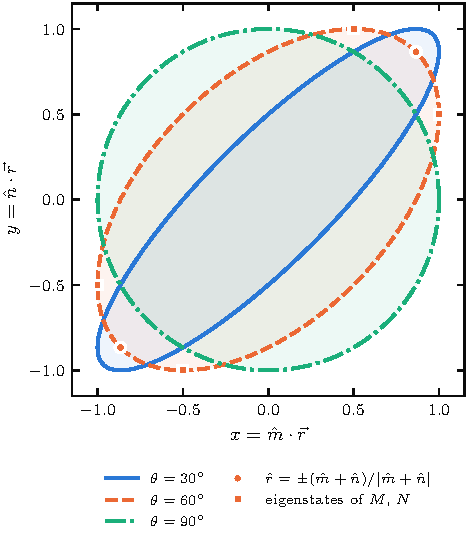
\includegraphics[width=0.48\linewidth]{achievable_set.pdf}
  \caption{\textbf{Achievable expectation values for two qubit measurements.}
  The ellipse $\mathcal E_\theta$ of achievable
  $(x,y)=(\langle\mhat\cdot\vsigma\rangle,\langle\nhat\cdot\vsigma\rangle)$ for three
  Bloch angles $\theta$. Markers ($\theta=60^\circ$) show the two families of
  states that saturate the partial sums of $\omplus$: eigenstates of $M$ or $N$
  (squares; $k=1,3$) and bisector states $\hat r\propto\pm(\mhat+\nhat)$ (circles;
  $k=2$). No single point saturates all partial sums (Proposition~\ref{prop:attain}).}
  \label{fig:ellipse}
\end{figure}

\subsection*{Optimal bounds and their non-attainment}

\begin{theorem}[Refs.~\citenum{RPZ2014,LiQiao2019}]\label{thm:dsum}
For projective qubit measurements with maximal overlap $c$,
\begin{equation}
  p(\rho)\oplus q(\rho)\maj\omplus:=\bigl(1,\ \sqc,\ 1-\sqc,\ 0\bigr)\qquad\forall\rho,
  \label{eq:omplus}
\end{equation}
and $\omplus$ is the optimal majorization bound.
\end{theorem}

\begin{theorem}[Refs.~\citenum{FGG2013,PRZ2013,Partovi2011}]\label{thm:tensor}
Under the same assumptions, $p(\rho)\otimes q(\rho)\maj\omtimes:=(w,1-w,0,0)$ for all
$\rho$, with $w=\frac14(1+\sqc)^2$, and $\omtimes$ is the optimal majorization
bound.
\end{theorem}

Both follow from Lemma~\ref{lem:ellipse} in a few lines (Methods). The
central partial sum of $\omplus$ is $S_2=1+\sqc$, the qubit case of the
Landau--Pollak-type inequality $p_i+q_j\le1+\sqc$ behind Deutsch's
relation\cite{Deutsch1983,LandauPollak1961}; for mutually unbiased bases
$\omtimes$ is the vector of Partovi\cite{Partovi2011}. The two families of
states that saturate the partial sums never coincide:

\begin{proposition}\label{prop:attain}
(i) A state with $(p\oplus q)^\downarrow=\omplus$ exists iff $c=1$, i.e., iff $M$
and $N$ commute. For $c<1$, $S_1$ and $S_3$ are attained only by eigenstates of
$M$ or $N$, and $S_2$ only by the bisector states $\vecr=\pm(\mhat+\nhat)/|\mhat+\nhat|$
(for $\theta=\pi/2$ also by $\pm(\mhat-\nhat)/|\mhat-\nhat|$).
(ii) A state with $(p\otimes q)^\downarrow=\omtimes$ exists iff $c=1$.
\end{proposition}

Demanding certainty about $M$ lowers the largest attainable $L_2(p\oplus q)$ from
$1+\sqc$ to $1+c$, a deficit $\sqc(1-\sqc)$ that vanishes only for commuting
measurements (Fig.~\ref{fig:lorenz}). The optimal vectors are therefore suprema
in the majorization lattice, not the statistics of any state, which makes
precise, for the binary case, the general remark of Partovi\cite{Partovi2011}.
Once the saturating states of the individual partial sums are known\cite{LiQiao2019},
the proof is short; its value lies in what follows from it.

\begin{figure}[t]
  \centering
  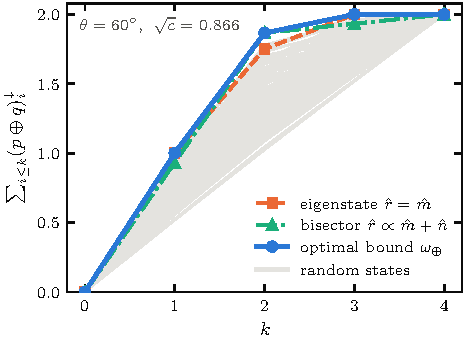
\includegraphics[width=0.48\linewidth]{lorenz.pdf}
  \caption{\textbf{The optimal bound is an envelope, not a state.} Lorenz curves
  of $p\oplus q$ for $\theta=60^\circ$. Grey: 150 random states. The optimal bound
  $\omplus$ (blue) is the smallest concave curve above all of them; it touches
  the eigenstate curve at $k=1,3$ and the bisector-state curve at $k=2$, but no
  single state reaches it.}
  \label{fig:lorenz}
\end{figure}

\subsection*{Consequences for entropic uncertainty}

Let $h(t)=-t\log_2t-(1-t)\log_2(1-t)$. Theorems~\ref{thm:dsum} and
\ref{thm:tensor} give the known bounds\cite{RPZ2014,FGG2013,PRZ2013}
\begin{align}
  &H(p)+H(q)\ge h(\sqc),\qquad
  T_\gamma(p)+T_\gamma(q)\ge\frac{1-c^{\gamma/2}-(1-\sqc)^\gamma}{\gamma-1},
  \label{eq:dsumbounds}\\
  &H_\alpha(p)+H_\alpha(q)\ge H_\alpha(\sqc,1-\sqc)\ \ (0<\alpha\le1),\qquad
  H_\alpha(p)+H_\alpha(q)\ge H_\alpha(\omtimes)\ \ (\alpha\in[0,\infty]).
  \label{eq:renyibounds}
\end{align}
For $\alpha\le1$ the direct-sum bound is the stronger one; that the direct-sum
form cannot be extended to all orders was stated in Ref.~\citenum{RPZ2014}, and
we make it explicit:

\begin{proposition}\label{prop:renyi}
(i) For $0<\alpha\le1$, $H_\alpha(\sqc,1-\sqc)\ge H_\alpha(\omtimes)$, with equality iff
$c=1$. (ii) For $c<1$ the direct-sum form fails at $\alpha=\infty$:
$\min_\rho[H_\infty(p)+H_\infty(q)]=-2\log_2\frac{1+\sqc}2<-\frac12\log_2c$.
\end{proposition}

The failure, however, sets in only beyond $\alpha=2$. Numerically, for qubits
$H_\alpha(\sqc,1-\sqc)$ is a valid bound for every $\alpha\le2$ at every angle, and
fails above an angle-dependent order between $2.00$ ($\theta\to0$) and $2.58$
($\theta\to90^\circ$). At $\alpha=2$, where the bisector state is optimal at every
angle\cite{ZozorBosykPortesi2013}, validity reduces to $(\sqc-1)^3(\sqc+3)\le0$
(Methods). The direct-sum form thus extends well beyond the range $\alpha\le1$
in which it is proven in general.

Non-attainment now has a sharp consequence.

\begin{theorem}\label{thm:strict}
Let $c<1$. (i) For every continuous, strictly Schur-concave $\Phi$,
$\min_\rho\Phi(p\oplus q)>\Phi(\omplus)$ and $\min_\rho\Phi(p\otimes q)>\Phi(\omtimes)$.
Hence the Shannon and Tsallis bounds in Eq.~\eqref{eq:dsumbounds} and the R\'enyi
bounds in Eq.~\eqref{eq:renyibounds} with $0<\alpha<\infty$ are all strict.
(ii) The tensor bounds of order $\alpha=0$ and $\alpha=\infty$ are tight, attained
by eigenstates and by bisector states, respectively.
\end{theorem}

The proof uses only that the achievable set is compact and that its supremum is
not attained, so it applies verbatim to every case below where the optimal
bound is not attained. As majorization bounds, $\omplus$ and $\omtimes$ cannot be
improved; as bounds on any single strictly Schur-concave measure, they always
can. For such measures the optimum must be found measure by measure, which is
what entropy-specific relations do.

\emph{How large is the gap?} The exact minimum of $H(p)+H(q)$ for two qubit
bases is known\cite{SanchezRuiz1998,Ghirardi2003}: it lies on the great circle
through $\mhat$ and $\nhat$, equals $2h(\frac{1+\sqc}2)$ at the bisector state for
$\theta\le\bar\theta$, where $\sqrt{\bar c}\artanh\sqrt{\bar c}=1$\cite{Bosyk2011},
i.e.\ $\bar\theta\approx67.07^\circ$, and moves continuously to the eigenstates,
reached at $\theta=90^\circ$, for larger angles. Figure~\ref{fig:shannon} compares
it with the majorization bounds and with MU, $H(p)+H(q)\ge-\log_2c$. Over all
angles $h(\sqc)$ is at least $78.2\%$ of the exact minimum (worst at
$\theta\approx70^\circ$; equivalently, the minimum exceeds the bound by up to
$28\%$), the largest absolute gap being $0.196$ bit at $\theta\approx74^\circ$; the
tensor bound $h(w)$ reaches at least $76.1\%$ of the minimum (at
$\theta\approx70.6^\circ$) and falls short by up to $0.217$ bit. At $\theta=90^\circ$, where MU
is tight, $h(\sqc)=0.872$ bit. Yet $h(\sqc)>-\log_2c$ for all $\theta<\theta^*\approx81.3^\circ$
($79.3^\circ$ for the tensor bound), the root of $h(\cos\frac\theta2)=-2\log_2\cos\frac\theta2$,
in agreement with the numerical observation of Ref.~\citenum{Baek2019}. As
$\theta\to0$, with $\varepsilon=1-\sqc\approx\theta^2/8$, one finds
$h(\sqc)\approx\varepsilon\log_2(e/\varepsilon)$ and an exact minimum
$2h(\varepsilon/2)\approx\varepsilon\log_2(2e/\varepsilon)$, so their ratio tends to one
as $1+1/\log_2(e/\varepsilon)$ (1.09 at $\theta=0.1$\,rad, 1.047 at $0.003$\,rad),
whereas the ratio of $h(\sqc)$ to MU grows as $\frac12\ln(8e/\theta^2)$. The
eigenstates, although they saturate $S_1$ and $S_3$, give $h(c)$, asymptotically
twice the minimum. For the Shannon entropy alone, the closed-form
bound\cite{SanchezRuiz1998,KTW2014} $h\bigl(\frac{1+\sqrt{2c-1}}2\bigr)$ is strictly
stronger than $h(\sqc)$ at every angle and at least as strong as MU, with which it
coincides at $90^\circ$ (0.601 against 0.568 bit for $h(\sqc)$ at $60^\circ$); what
majorization offers instead is one bound for all Schur-concave measures.

\begin{figure}[t]
  \centering
  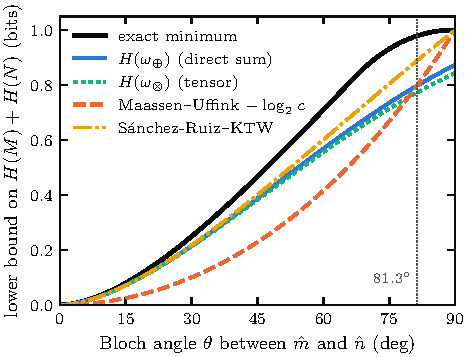
\includegraphics[width=0.6\linewidth]{entropic_bounds.pdf}
  \caption{\textbf{The price of universality for the Shannon entropy.} Lower
  bounds on $H(M)+H(N)$ versus the Bloch angle $\theta$ ($c=\cos^2\frac\theta2$).
  Black: exact minimum, equal to $2h(\frac{1+\sqc}2)$ for
  $\theta\le\bar\theta\approx67.07^\circ$. Blue: direct-sum bound $h(\sqc)$.
  Green (dotted): tensor-product bound $h(w)$. Orange (dashed): Maassen--Uffink.
  Yellow (dash-dotted): the closed-form Shannon bound
  $h(\frac{1+\sqrt{2c-1}}2)$\cite{SanchezRuiz1998,KTW2014}, strictly above $h(\sqc)$
  and at least as strong as MU. The direct-sum bound beats MU for $\theta<81.3^\circ$ (dotted line).}
  \label{fig:shannon}
\end{figure}

Figure~\ref{fig:renyi} extends the comparison to the R\'enyi family. For
$\alpha\le1$ MU also applies, since $H_\alpha$ is non-increasing in $\alpha$. At
$\theta=60^\circ$ both majorization bounds beat MU for all $\alpha\le1$; at
$\theta=85^\circ$ only for $\alpha<0.69$ (direct sum) and $\alpha<0.58$ (tensor). For
the max-entropy the direct-sum bound reaches $83\%$ and $91\%$ of the exact
minimum at the two angles. For large $\alpha$ only the tensor bound remains, and
it converges to the exact minimum as $\alpha\to\infty$, as Theorem~\ref{thm:strict}
requires. Which state is optimal depends on the measure\cite{ZozorBosykPortesi2013,LuisBosykPortesi2016,KorzekwaLostaglio2016}:
for $c>\frac12$ the eigenstates are optimal for $\alpha\le\alpha_0(c)$ and the
bisector for $\alpha\ge\alpha^\star(c)$, with intermediate states in between. Here
$\alpha_0$ exceeds $\frac12$ (0.52, 0.56 and 0.66 at $20^\circ$, $60^\circ$ and
$85^\circ$), and $\alpha^\star$ rises from $\frac12$ as $c\to1$ to
$\alpha^\dagger\approx1.43$ as $c\to\frac12$\cite{ZozorBosykPortesi2013}; the
bisector is optimal up to $43^\circ$ for $\alpha=\frac34$, up to $\bar\theta$ for
the Shannon entropy, up to $80^\circ$ for $\alpha=1.2$ and at all angles for
$\alpha\ge\alpha^\dagger$, consistent with the tightness of the min-entropy bound.

\begin{figure}[t]
  \centering
  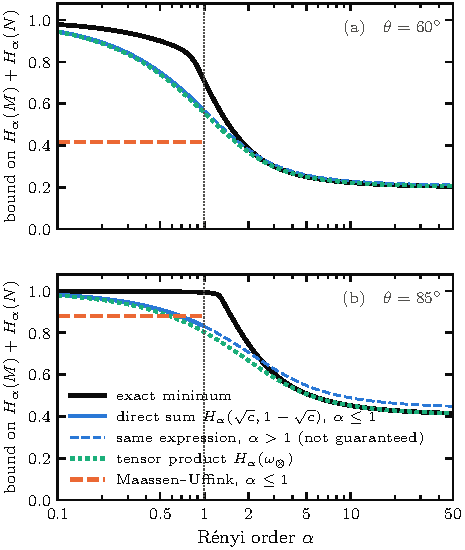
\includegraphics[width=0.55\linewidth]{renyi_family.pdf}
  \caption{\textbf{Bounds across the R\'enyi family.} Bounds on
  $H_\alpha(M)+H_\alpha(N)$ for (a) $\theta=60^\circ$ and (b) $\theta=85^\circ$. Black:
  exact minimum. Blue: direct-sum bound $H_\alpha(\sqc,1-\sqc)$, proven for
  $\alpha\le1$; its thin dashed continuation for $\alpha>1$ remains a valid bound up to
  $\alpha=2$ but exceeds the exact minimum above $\alpha\approx2.1$ in (a) and
  $\alpha\approx2.5$ in (b). Green (dotted): tensor-product bound
  $H_\alpha(\omtimes)$. Orange (dashed): MU, valid for $\alpha\le1$. Dotted
  vertical line: Shannon case $\alpha=1$.}
  \label{fig:renyi}
\end{figure}

\subsection*{Noisy and biased measurements}

For POVMs, the partial sums of the direct-sum relation are largest eigenvalues
of sums of effects\cite{Baek2019,RPZ2014,RasteginZyczkowski2016,Bosyk2014},
$S_k=\max_{|J|=k}\lambda_{\max}\bigl(\sum_{j\in J}K_j\bigr)$, with the $K_j$ running
over the effects of both measurements; the flattened vector they define is
optimal for general measurements\cite{Yuan2023}. For two-outcome qubit POVMs, whose
achievable expectation values were described geometrically in
Ref.~\citenum{Abbott2016}, the maximization can be done in closed form for
arbitrary bias, and no flattening is needed. Let $M$ have parameters $(\mu,\eta,\hat a)$ and $N$ parameters
$(\nu,\zeta,\hat b)$ in Eq.~\eqref{eq:povm}.

\begin{theorem}\label{thm:povm}
Define
\begin{equation}
  \kappa=\max\{|\mu|+\eta,\ |\nu|+\zeta\},\qquad
  \Lambda=\max_{s,t=\pm1}\bigl[s\mu+t\nu+|s\eta\hat a+t\zeta\hat b|\bigr].
  \label{eq:kappaLambda}
\end{equation}
Then $p(\rho)\oplus q(\rho)\maj\omplus(M,N)$ for all $\rho$, where
\begin{equation}
  \omplus(M,N)=\tfrac12\bigl(1+\kappa,\ 1+\Lambda-\kappa,\ 1+\kappa-\Lambda,\ 1-\kappa\bigr)
  \label{eq:omplusPOVM}
\end{equation}
is the optimal majorization bound; $S_1=\frac12(1+\kappa)$ and $S_2=1+\frac12\Lambda$.
\end{theorem}

For projective measurements $\kappa=1$, $\Lambda=2\sqc$, and Eq.~\eqref{eq:omplus}
is recovered; for unbiased ones $\Lambda=(\eta^2+\zeta^2+2\eta\zeta|\hat a\cdot\hat b|)^{1/2}$,
in agreement with Ref.~\citenum{Baek2019}. With unequal sharpness or bias the
relevant geometric quantities are the lengths $|\eta\hat a\pm\zeta\hat b|$ rather
than $c$, and the bound is the qubit case of Corollary~\ref{cor:povmd} below.
Theorem~\ref{thm:povm} also covers states of fixed spectrum: projective
measurements on states with $|\vecr|=r$ have the statistics of unbiased
measurements of sharpness $\eta=\zeta=r$ on pure states, so the spectrum-dependent
bound\cite{LiQiao2019,Puchala2018} is
$\frac12(1+r,\,1-r+2r\sqc,\,1+r-2r\sqc,\,1-r)$, and by Proposition~\ref{prop:povmattain}
below it is not attained for $r>0$ and $c<1$.

\begin{proposition}\label{prop:povmattain}
(i) If $E_0$ and $F_0$ do not commute, $\eta\zeta\,\hat a\times\hat b\ne0$, no
state attains $\omplus(M,N)$. (ii) If $\mu=\nu=0$ and $E_0$, $F_0$ commute, a state
attains it. (iii) With bias, commuting effects need not attain it: for
$\hat b=\hat a$, $(\mu,\eta)=(0.3,0.6)$ and $(\nu,\zeta)=(-0.8,0.15)$, $S_1$ is
attained only at $\vecr=-\hat a$ and $S_2$ only at $\vecr=\hat a$.
\end{proposition}

By Theorem~\ref{thm:strict}, $H(p)+H(q)\ge-\sum_k\omega_k\log_2\omega_k$ with
$\omega=\omplus(M,N)$ is therefore strict whenever the effects do not commute.
Figure~\ref{fig:povm} shows that it tracks the exact minimum as functions of
sharpness and of bias. The example in (iii), two readouts of the same axis
favouring opposite ends of it, is a trade-off of purely classical origin.
Attainment is also unrelated to joint measurability: unbiased POVMs are jointly
measurable iff $|\eta\hat a+\zeta\hat b|+|\eta\hat a-\zeta\hat b|\le2$\cite{Busch1986,HMZ2016}
(the biased criterion is more involved\cite{StanoReitznerHeinosaari2008,BuschSchmidt2010,Yu2010});
for orthogonal axes and $\eta=\zeta\le1/\sqrt2$ the pair is jointly measurable,
yet $S_2=1+\eta/\sqrt2<1+\eta$ and the bound is not attained. Majorization
uncertainty relations thus quantify preparation uncertainty, which persists
without measurement incompatibility.

\begin{figure}[t]
  \centering
  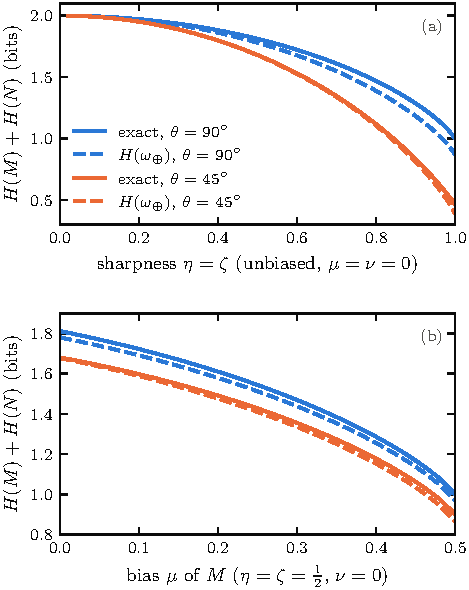
\includegraphics[width=0.48\linewidth]{povm.pdf}
  \caption{\textbf{Noisy and biased qubit measurements.} Exact minimum of
  $H(M)+H(N)$ (solid) and the bound from Theorem~\ref{thm:povm} (dashed) for
  Bloch angles $90^\circ$ and $45^\circ$. (a) Unbiased measurements of equal
  sharpness ($\mu=\nu=0$, $\eta=\zeta$). (b) $M$ with sharpness $\eta=\frac12$ and
  bias $\mu$; $N$ unbiased with $\zeta=\frac12$.}
  \label{fig:povm}
\end{figure}

\subsection*{Imperfect detectors and uncertainty-based tests}

Bias and unequal sharpness are what real detectors produce. If the two outputs
of a polarizing beam splitter are monitored by detectors of efficiencies
$\eta_H$ and $\eta_V$ and no-click events are assigned to either outcome at
random, the effect of outcome $H$ has the form~\eqref{eq:povm} with
$\mu=(\eta_H-\eta_V)/2$ and $\eta=(\eta_H+\eta_V)/2$; a mismatch of efficiencies, a
known concern in quantum key distribution\cite{Makarov2006}, appears as a bias.
A single click/no-click detector behind a polarizer, with no-click counted as
the second outcome, gives $E_0=\eta_dP$, i.e.\ $\mu=\eta_d-1$, $\eta=\eta_d$ and
$|\mu|+\eta=1$. Experiments that test uncertainty relations, or use them to
certify entanglement or steering, usually compare data with the bound for ideal
measurements. Theorem~\ref{thm:povm} tells exactly when this is justified.

\begin{proposition}\label{prop:detectors}
Let $M,N$ be two-outcome qubit POVMs with axes $\hat a,\hat b$, let
$M^\circ,N^\circ$ be the projective measurements along the same axes, with
statistics $p^\circ,q^\circ$ and overlap $c=\frac12(1+|\hat a\cdot\hat b|)<1$.
(i) If $\mu=\nu=0$, then $p(\rho)\oplus q(\rho)\maj p^\circ(\rho)\oplus q^\circ(\rho)$
for every $\rho$; hence every lower bound on $\Phi(p\oplus q)$ or on $\Phi(p)+\Psi(q)$,
with $\Phi,\Psi$ Schur-concave, that holds for $M^\circ,N^\circ$ also holds for
$M,N$.
(ii) In general, the ideal relation $p(\rho)\oplus q(\rho)\maj\omplus=(1,\sqc,1-\sqc,0)$
holds for all $\rho$ iff $\Lambda\le2\sqc$. If $\Lambda>2\sqc$, some state violates the
Landau--Pollak relation $p_i+q_j\le1+\sqc$ of the ideal measurements.
(iii) If $M$ and $N$ are read out by the same detectors, $\mu=\nu$ and
$\eta=\zeta$, with $\hat a\cdot\hat b\ge0$, the condition reads
$|\mu|\le\sqc\,(1-\eta)$. Click/no-click detection violates it for every
$\eta_d<1$.
\end{proposition}

Noise only blurs the statistics towards the uniform distribution, but bias
shifts the image of $\mathcal E_\theta$, and the shifted ellipse can leave the
ideal one. Whether a particular entropic bound is violated depends on the
measure: the Shannon minimum is more forgiving than the Landau--Pollak sum, but
not immune (Fig.~\ref{fig:detectors}). For orthogonal axes and random no-click
assignment, an efficiency $\eta_H=0.99$ violates the ideal relation for
$\eta_V<0.942$ and the ideal Shannon bound of one bit for $\eta_V<0.578$; for
$\eta_H=0.95$ the thresholds are $0.708$ and $0.211$, and for $\eta_H\le0.9$ the
Shannon bound is never violated, although the ideal relation still is for
$\eta_V<0.417$. Click/no-click detectors lower the Shannon minimum below its
ideal value at all efficiencies and angles we examined; for orthogonal axes this
holds for every $\eta_d<1$, since the eigenstate of the dark outcome of $M$ gives
$H(M)+H(N)=h(\eta_d/2)<1$. In all
cases $H(\omplus(M,N))$ remains a valid bound.

This matters for steering tests\cite{Walborn2011,Schneeloch2013,Uola2020}, in
which Bob trusts his measurements and Alice's are uncharacterized.

\begin{corollary}\label{cor:steering}
If Alice's measurements $A_1,A_2$ and Bob's two-outcome measurements $M,N$
admit a local-hidden-state model, then
\begin{equation}
  H(M|A_1)+H(N|A_2)\ \ge\ \min_\rho\bigl[H(M)+H(N)\bigr]\ \ge\ H\bigl(\omplus(M,N)\bigr).
  \label{eq:steering}
\end{equation}
The minimum for the ideal measurements $M^\circ,N^\circ$ may replace the right-hand
side if $M,N$ are unbiased, but not in general: for click/no-click detection
along orthogonal axes, a product state with Bob in the dark eigenstate of $M$
gives $H(M|A_1)+H(N|A_2)=h(\eta_d/2)$, below the ideal value of one bit for every
$\eta_d<1$.
\end{corollary}

An uncertainty-based steering or entanglement test with biased trusted
detectors must therefore use the bound of the measurements actually performed;
Theorem~\ref{thm:povm} provides it in closed form, for every Schur-concave
measure at once, and Proposition~\ref{prop:detectors} tells when the ideal bound
can be kept.

\begin{figure}[t]
  \centering
  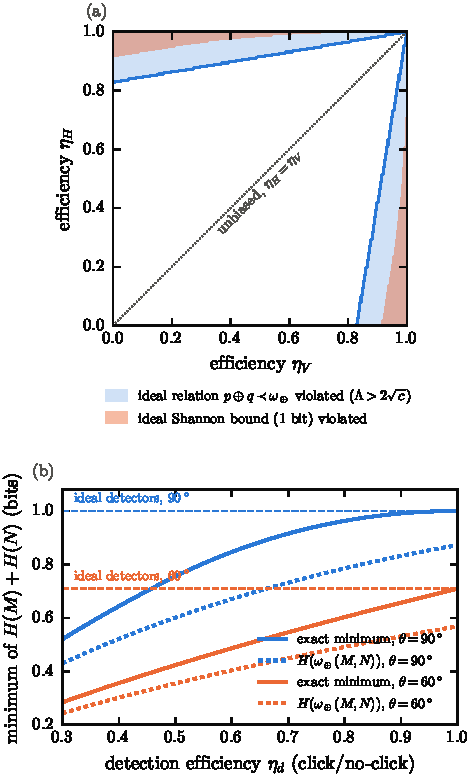
\includegraphics[width=0.48\linewidth]{detector_bias.pdf}
  \caption{\textbf{Detector bias can invalidate ideal-detector uncertainty
  bounds.} (a) Polarizing beam splitter with detectors of efficiencies
  $(\eta_H,\eta_V)$ and random assignment of no-click events, for measurements
  along orthogonal axes read out by the same detectors. Blue: the ideal
  relation $p\oplus q\maj\omplus$ fails ($\Lambda>2\sqc$, Proposition~\ref{prop:detectors});
  orange: the ideal Shannon bound of one bit fails. Unbiased detectors
  ($\eta_H=\eta_V$, dotted) never violate ideal bounds. (b) Click/no-click
  detection with efficiency $\eta_d$: exact minimum of $H(M)+H(N)$ (solid) and
  the bound $H(\omplus(M,N))$ of Theorem~\ref{thm:povm} (dotted) for Bloch angles
  $90^\circ$ and $60^\circ$; dashed lines mark the minimum for ideal detectors.}
  \label{fig:detectors}
\end{figure}

\subsection*{Binary measurements in any finite dimension}

\begin{theorem}\label{thm:dimd}
Let $M=\{P,\mathbb 1-P\}$ and $N=\{Q,\mathbb 1-Q\}$ be projective measurements on
$\mathbb C^d$, write $P_1=P$, $P_2=\mathbb 1-P$, $Q_1=Q$, $Q_2=\mathbb 1-Q$, and let
$c=\max_{i,j}\|P_iQ_j\|^2$. Then Theorems~\ref{thm:dsum} and \ref{thm:tensor} hold
verbatim, and $\omplus$ and $\omtimes$ are attained iff $c=1$.
\end{theorem}

The direct-sum part follows from the eigenvalue formula\cite{Baek2019} and
$\lambda_{\max}(P+Q)=1+\|PQ\|$\cite{Halmos1969}, and the tensor part from the reduction to
qubit blocks by Jordan's lemma\cite{Halmos1969,KTW2014}; new are the tensor bound and
the attainment conditions in dimension $d$. The overlap has the operator form
$c=\frac12+\frac14\|\{A,B\}\|$ with $A=2P-\mathbb 1$, $B=2Q-\mathbb 1$, as shown in any
dimension by Kaniewski \emph{et al.}\cite{KTW2014}, closely related to the formula
$\|PQ+QP\|=\|PQ\|+\|PQ\|^2$\cite{Walters2016}. All results of the previous
sections therefore hold for binary projective measurements in any dimension;
the min-entropy bound remains tight, and for $c<1$ the bounds for strictly
Schur-concave measures are strict. The direct-sum argument uses only the
eigenvalue formula and carries over to noisy and biased measurements:

\begin{corollary}\label{cor:povmd}
Let $M=\{E_1,E_2\}$ and $N=\{F_1,F_2\}$ be two-outcome POVMs on $\mathbb C^d$, let $S_1$
be the largest eigenvalue of the four effects and
$S_2=\max_{i,j}\lambda_{\max}(E_i+F_j)$. Then
\begin{equation}
  p(\rho)\oplus q(\rho)\maj\bigl(S_1,\ S_2-S_1,\ 1+S_1-S_2,\ 1-S_1\bigr)\qquad\forall\rho,
  \label{eq:povmd}
\end{equation}
and this vector is the optimal majorization bound.
\end{corollary}

Theorem~\ref{thm:povm} is the qubit case, $S_1=\frac12(1+\kappa)$ and
$S_2=1+\frac12\Lambda$, and Theorem~\ref{thm:dimd} the projective case, $S_1=1$
and $S_2=1+\sqc$. Part (ii) of Proposition~\ref{prop:detectors} generalizes in the
same way: since $S_1\le1$ and $S_3=1+S_1\le2$ always, two binary POVMs obey the
relation $p\oplus q\maj(1,\sqc,1-\sqc,0)$ of a reference pair of projective
measurements with overlap $c$ iff $S_2\le1+\sqc$.

% ===========================================================================
\section*{Discussion}
% ===========================================================================

For binary measurements the majorization approach to uncertainty can be carried
out completely. The achievable statistics of a qubit are an affine image of an
ellipse, and a single four-component vector, determined by the overlap $c$, is
their least upper bound in the majorization lattice, for the direct sum as well
as for the tensor product; for POVMs it is determined by $\kappa$ and $\Lambda$, and
in any dimension by the largest eigenvalues of the effects and of their pairwise
sums. One vector controls every Schur-concave uncertainty measure at once.

The price of this unification is now precise. Because the supremum is not the
statistics of any state unless the measurements commute, the induced bound is
strict for every strictly Schur-concave measure and exact only at R\'enyi orders
zero and infinity. Quantitatively the price is moderate where it matters most:
the direct-sum Shannon bound is never below $78\%$ of the exact value, beats MU
for Bloch angles below $81.3^\circ$, and becomes asymptotically tight in ratio as
the measurements approach compatibility, precisely where MU is weakest. Where
only one measure matters, as for the Shannon entropy in the analysis of key
distribution, the entropy-specific optimum should be used; where many matter at
once, or where the measure is not fixed in advance, majorization gives the only
universal bound, and we now know how far from tight it is.

The second lesson concerns imperfect measurements. Majorization makes the
distinction between noise and bias sharp: noise acts as a doubly stochastic map
on the statistics and can only increase every measure of uncertainty, whereas
bias moves the achievable set. Whether ideal-detector relations survive is
decided by one partial sum, $S_2$, that is, by $\Lambda\le2\sqc$ for qubits.
Uncertainty-based tests of entanglement and steering with trusted detectors
must therefore account for detector bias explicitly, as they do for losses in
other contexts; the closed-form bound of Theorem~\ref{thm:povm} does so for all
Schur-concave measures simultaneously. Non-attainment is itself testable: experiments
have reported Lorenz curves that touch the optimal bound\cite{Wang2020}, which by
Proposition~\ref{prop:attain} can only happen for individual partial sums, and the
distance $\min_\rho\max_k[S_k-L_k(p\oplus q)]$ between the bound and the closest state is
a directly measurable quantity. A natural next step is an experimental
test with deliberately mismatched detectors, for instance in the
coherent-light\cite{Wang2020} or photonic\cite{Yuan2023} settings in which
optimal majorization bounds have already been probed.

\emph{Relation to quantum optics.} For the quadratures of a light mode, coherent
and squeezed states saturate both the Heisenberg relation and the entropic
relation of Bia{\l}ynicki-Birula and Mycielski\cite{BBM1975}, and pure Gaussian
states are conjectured to majorize every Wigner-positive state\cite{VanHerstraeten2023}.
For non-commuting binary measurements no such state exists
(Propositions~\ref{prop:attain} and \ref{prop:povmattain}), and the optimal state
depends on the measure\cite{KorzekwaLostaglio2016,LuisBosykPortesi2016}. The
boundary of $\mathcal E_\theta$ plays the role of the squeezed-state family, and the
balanced bisector state that of a coherent state, which minimizes the Shannon
sum up to $\bar\theta\approx67^\circ$. The difference is algebraic: for quadratures
the commutator is a c-number, whereas for binary observables the anticommutator
is, blockwise, a c-number, and it fixes $c=\frac12+\frac14\|\{A,B\}\|$. The Robertson
bound vanishes for every state in the plane of the two axes, which contains all
optimal states; the missing information is carried by the anticommutator term
of the Robertson--Schr\"odinger relation, which every pure state saturates
(Methods). For single photons, two linear polarization analysers at relative
angle $\vartheta$ give $\theta=2\vartheta$ and $c=\cos^2\vartheta$ (Malus's law); the
crossover with MU and the angle $\bar\theta$ correspond to $\vartheta\approx40.7^\circ$ and
$33.5^\circ$.

\emph{Open questions.} (i) The optimal tensor-product bound for noisy or biased
measurements: already for unbiased measurements of equal sharpness $S_3$ is
attained neither by eigenstates nor by bisector states. (ii) A closed form for
$\lambda_{\max}(E_i+F_j)$ in Corollary~\ref{cor:povmd}, analogous to
$1+\|P_iQ_j\|$ for projectors, and attainment conditions in dimension $d$.
(iii) More than two measurements: for qubit bases
$S_k=\frac k2+\frac12\max_J|\sum_{j\in J}\vec n_j|$, and Li and Qiao obtained the optimal
bound for $\sigma_x,\sigma_y,\sigma_z$\cite{LiQiao2019}; for random triples we always
found the increments ordered, but have no proof. (iv) Whether state-independent
relations of the form~\eqref{eq:MUR} can reproduce mixed-order relations such as
$H_\infty(p)+H_{1/2}(q)\ge-\log_2c$, which conditional majorization yields for
qubits\cite{XiaoFangGour2019}. (v) Binary measurements on light modes: for
photon-number parity and displaced parity, or for coherent-state tests realized
by displacement and on/off detection, $c=1$ without a common eigenvector, so no
non-trivial state-independent relation exists, although individual partial sums
remain informative; for coherent-state tests
$\pi[Q(\nu_1)+Q(\nu_2)]\le1+e^{-|\nu_1-\nu_2|^2/2}$, with equality for an optical cat
state\cite{Ourjoumtsev2007,Lewenstein2021}, which plays the role of the bisector
state. Non-trivial relations require $\|\{A,B\}\|<2$, as for pseudospin
operators\cite{Chen2002} or polarization measurements on single photons.

% ===========================================================================
\section*{Methods}
% ===========================================================================

\subsection*{Proof of Lemma~\ref{lem:ellipse} and the covariance form}

Write $\vecr=\vecr_\parallel+\vecr_\perp$ with $\vecr_\parallel\in\operatorname{span}\{\mhat,\nhat\}$.
Only $\vecr_\parallel$ contributes to $(x,y)=G\xi$, where $\xi$ are the coefficients of
$\vecr_\parallel$ in the basis $\{\mhat,\nhat\}$ and $G=\bigl(\begin{smallmatrix}1&\cos\theta\\
\cos\theta&1\end{smallmatrix}\bigr)$ is the Gram matrix. Then
$|\vecr_\parallel|^2=\xi^TG\xi=(x,y)G^{-1}(x,y)^T\le1$, which is Eq.~\eqref{eq:ellipse} since
$\det G=\sin^2\theta$; equality holds iff $\vecr_\perp=0$ and $|\vecr|=1$. Conversely every
$(x,y)\in\mathcal E_\theta$ is attained by $\vecr=\xi_1\mhat+\xi_2\nhat$ with
$\xi=G^{-1}(x,y)^T$. The support function is Cauchy--Schwarz:
$sx+ty=\vecr\cdot(s\mhat+t\nhat)$. The covariance matrix of $A,B$ is
$\Gamma=\bigl(\begin{smallmatrix}1-x^2&\cos\theta-xy\\\cos\theta-xy&1-y^2\end{smallmatrix}\bigr)$
and $\det\Gamma=\sin^2\theta-(x^2-2xy\cos\theta+y^2)$, so $(x,y)\in\mathcal E_\theta$ iff
$\Gamma\ge0$. The Robertson--Schr\"odinger relation reads
$\det\Gamma\ge\langle(\mhat\times\nhat)\cdot\vsigma\rangle^2$; for a pure state
$\langle(\mhat\times\nhat)\cdot\vsigma\rangle^2=\sin^2\theta-(x^2-2xy\cos\theta+y^2)$, so pure
states saturate it, and in the plane of the axes it reduces to the boundary
$\det\Gamma=0$.

\subsection*{Proofs of Theorems~\ref{thm:dsum} and \ref{thm:tensor}}

\emph{Direct sum.} Clearly $S_1\le1$ and $S_4=2$; since all entries are
non-negative, $S_3=2-\min_\rho\min_i(p\oplus q)_i\le2$, and both bounds are attained by
an eigenstate of $M$. For $k=2$ the two largest entries either belong to the
same distribution, with sum 1, or are of the form
$p_i+q_j=1+\frac12(\pm x\pm y)\le1+\frac12\max\{|\mhat+\nhat|,|\mhat-\nhat|\}$ by
Lemma~\ref{lem:ellipse}. With $\mhat\cdot\nhat\ge0$ the maximum is
$|\mhat+\nhat|=2\cos\frac\theta2=2\sqc$, so $S_2=1+\sqc$, attained by the bisector state.
The increments of $(1,1+\sqc,2,2)$ give $\omplus$, which is non-increasing because
$1\ge\sqc\ge1-\sqc$ (as $c\ge\frac12$); Lemma~\ref{lem:sup} completes the proof.

\emph{Tensor product.} By the arithmetic--geometric mean inequality and
$S_2=1+\sqc$, $p_iq_j\le(\frac{p_i+q_j}2)^2\le(\frac{1+\sqc}2)^2=w$, with equality at the
bisector state, where $p_+=q_+=(1+\sqc)/2$. Hence $S_1=w$. For an eigenstate of $M$,
$p\otimes q=(q_+,q_-,0,0)$, so $S_2=S_3=S_4=1$. Since $\sqc\ge1/\sqrt2$, $w\ge\frac12$
and the increments $(w,1-w,0,0)$ are non-increasing.

\subsection*{Proof of Proposition~\ref{prop:attain}}

(i) $(p\oplus q)^\downarrow_1=1$ forces an eigenstate of $M$ or $N$, say $\vecr=\pm\mhat$.
Then $q=(\frac{1\pm\cos\theta}2,\frac{1\mp\cos\theta}2)$ and $(p\oplus q)^\downarrow=(1,c,1-c,0)$,
which equals $\omplus$ iff $c=\sqc$, i.e.\ $c=1$. The statement about $S_2$ follows
from the equality condition in Cauchy--Schwarz and from $|\mhat-\nhat|<|\mhat+\nhat|$
for $\theta<\pi/2$. (ii) If $c=1$, a common eigenstate gives $p\otimes q=(1,0,0,0)=\omtimes$.
If $c<1$, $L_2(p\otimes q)=1=L_2(\omtimes)$ requires two vanishing entries of $p\otimes q$,
hence an eigenstate of $M$ or $N$, at which $L_1(p\otimes q)=c<w=L_1(\omtimes)$, since
$w-c=\frac14(1-\sqc)(1+3\sqc)>0$.

\subsection*{Proofs of the entropic bounds and Proposition~\ref{prop:renyi}}

Eq.~\eqref{eq:dsumbounds} is Karamata's inequality applied to Theorem~\ref{thm:dsum}
with $\phi(t)=-t\log_2t$ and $\phi_\gamma(t)=(t-t^\gamma)/(\gamma-1)$, using
$\sum_ip_i=\sum_jq_j=1$. For the direct-sum R\'enyi bound with $\alpha<1$, write
$\sum_ip_i^\alpha=1+X$, $\sum_jq_j^\alpha=1+Y$ with $X,Y\ge0$; then
$H_\alpha(p)+H_\alpha(q)=\frac{\log_2[(1+X)(1+Y)]}{1-\alpha}\ge\frac{\log_2(1+X+Y)}{1-\alpha}$ and
$1+X+Y=\sum_k(p\oplus q)_k^\alpha-1\ge\sum_k(\omplus)_k^\alpha-1=c^{\alpha/2}+(1-\sqc)^\alpha$ by
Schur-concavity\cite{RPZ2014}. The tensor bounds follow from
$H_\alpha(p)+H_\alpha(q)=H_\alpha(p\otimes q)$\cite{FGG2013,PRZ2013}; for $\alpha=\infty$ the bound
$-2\log_2\frac{1+\sqc}2$ is attained at the bisector state and contains Deutsch's
Shannon bound\cite{Deutsch1983}. Proposition~\ref{prop:renyi}(i): since
$w-\sqc=\frac14(1-\sqc)^2\ge0$, $(\sqc,1-\sqc)\maj(w,1-w)$ with equality iff $c=1$; apply
strict Schur-concavity. (ii): with $t=\sqc$, $(\frac{1+t}2)^2-t=(\frac{1-t}2)^2>0$
for $t<1$, and the minimum is the tight tensor bound.
\emph{Validity at $\alpha=2$.} With the bisector optimal\cite{ZozorBosykPortesi2013} and
$s=\sqc$, $a=\frac{1+s}2$, the exact minimum is $-2\log_2[a^2+(1-a)^2]=-2\log_2\frac{1+s^2}2$,
and $H_2(s,1-s)=-\log_2[s^2+(1-s)^2]$. The bound holds iff
$(\frac{1+s^2}2)^2\le s^2+(1-s)^2$, i.e.\ iff $\frac14(s-1)^3(s+3)\le0$, which is true for $s\le1$.

\subsection*{Proof of Theorem~\ref{thm:strict}}

(i) The achievable statistics form a compact set, so the minimum of $\Phi$ is
attained at some $\rho^*$. By Theorem~\ref{thm:dsum} and
Proposition~\ref{prop:attain}(i), $p\oplus q(\rho^*)\maj\omplus$ with
$(p\oplus q)^\downarrow\ne\omplus$, hence $\Phi(p\oplus q(\rho^*))>\Phi(\omplus)$; the tensor case
is analogous. The Shannon and Tsallis sums are strictly Schur-concave functions
of $p\oplus q$, and $H_\alpha(p)+H_\alpha(q)=H_\alpha(p\otimes q)$ with $H_\alpha$ strictly
Schur-concave for $0<\alpha<\infty$. For the direct-sum R\'enyi bound with $\alpha<1$,
apply the argument to $v\mapsto\sum_kv_k^\alpha$. (ii) An eigenstate of $M$ gives
$H_0(p)+H_0(q)=1=H_0(\omtimes)$, and a bisector state gives $\max_ip_i\max_jq_j=w$.

\subsection*{Proof of Theorem~\ref{thm:povm}}

The largest single outcome probability is
$\max_\rho\frac12(1+|\mu+\eta\hat a\cdot\vecr|)=\frac12(1+|\mu|+\eta)$ for $M$, so
$S_1=\frac12(1+\kappa)$; likewise the smallest is $\frac12(1-\kappa)$, so
$S_3=2-\frac12(1-\kappa)$. For $S_2$, a pair within one distribution sums to 1,
while a cross pair gives, by Cauchy--Schwarz,
$\max_\rho\bigl[1+\frac12\bigl(s(\mu+\eta\hat a\cdot\vecr)+t(\nu+\zeta\hat b\cdot\vecr)\bigr)\bigr]
=1+\frac12\bigl[s\mu+t\nu+|s\eta\hat a+t\zeta\hat b|\bigr]$. Choosing $s=\operatorname{sgn}\mu$,
$t=\operatorname{sgn}\nu$ shows $\Lambda\ge0$, so $S_2=1+\frac12\Lambda$. The increments of $(S_k)$ are
the entries of Eq.~\eqref{eq:omplusPOVM}; they are non-increasing iff
$\kappa\le\Lambda\le2\kappa$. The upper inequality follows from the triangle inequality,
$\Lambda\le|\mu|+|\nu|+\eta+\zeta\le2\kappa$. For the lower one, let $\rho^*$ attain $S_1$ via
an outcome of, say, $M$; then $S_2\ge S_1+\max_jq_j(\rho^*)\ge S_1+\frac12$, i.e.\
$\Lambda\ge\kappa$. Lemma~\ref{lem:sup} completes the proof.

\subsection*{Proof of Proposition~\ref{prop:povmattain}}

(i) Suppose a state attains $S_1$ through an outcome of $M$, so that $\kappa=|\mu|+\eta$
(the case of $N$ is symmetric). Since $\eta>0$, this forces $\vecr=s_0\hat a$ with
$s_0\mu=|\mu|$. There the two largest entries of $p\oplus q$ sum to
$1+\frac12\max_t[|\mu|+\eta+t\nu+ts_0\zeta\,\hat a\cdot\hat b]$, whereas the term $s=s_0$ of $\Lambda$
gives $S_2\ge1+\frac12[|\mu|+t\nu+|\eta\hat a+ts_0\zeta\hat b|]$ for each $t$. By
Cauchy--Schwarz, $|\eta\hat a+ts_0\zeta\hat b|>\eta+ts_0\zeta\,\hat a\cdot\hat b$ unless $\hat b=\pm\hat a$ (and $\eta\pm ts_0\zeta\ge0$), which is excluded when
$E_0$ and $F_0$ do not commute, so no state attains both $S_1$ and $S_2$.
(ii) If $\eta=0$, then $\Lambda=\kappa=\zeta$ and $\vecr=\hat b$ attains the bound.
Otherwise, up to relabelling the outcomes of $N$, $\hat b=\hat a$, so $\Lambda=\eta+\zeta$,
$\kappa=\max\{\eta,\zeta\}$, and $\vecr=\hat a$ gives
$(p\oplus q)^\downarrow=\frac12(1+\kappa,1+\Lambda-\kappa,1+\kappa-\Lambda,1-\kappa)$. (iii) Here $\kappa=0.95$ is
reached only by the second outcome of $N$ at $\vecr=-\hat a$, and $\Lambda=1.55$ only by
$(s,t)=(1,-1)$ at $\vecr=\hat a$.

\subsection*{Proof of Proposition~\ref{prop:detectors} and Corollary~\ref{cor:steering}}

(i) For $\mu=0$, $p=\eta p^\circ+(1-\eta)u$ with $u=(\frac12,\frac12)$, i.e.\ $p=Dp^\circ$ for the
doubly stochastic matrix $D=\frac12\bigl(\begin{smallmatrix}1+\eta&1-\eta\\1-\eta&1+\eta\end{smallmatrix}\bigr)$;
likewise $q=D'q^\circ$. Hence $p\maj p^\circ$, $q\maj q^\circ$ and, since $D\oplus D'$ is doubly
stochastic, $p\oplus q\maj p^\circ\oplus q^\circ$\cite{MarshallOlkin2011}. Schur-concavity gives the
claim. (ii) By Theorems~\ref{thm:dsum} and \ref{thm:povm} both $\omplus$ and $\omplus(M,N)$
are lattice suprema. If $\omplus(M,N)\maj\omplus$, transitivity gives
$p\oplus q\maj\omplus$ for all states; conversely, if $\omplus$ is an upper bound of all
$p\oplus q$, then $\omplus(M,N)=\sup\maj\omplus$. Comparing ordered partial sums,
$S_1=\frac12(1+\kappa)\le1$ and $S_3=\frac12(3+\kappa)\le2$ always hold, so the relation holds
iff $S_2=1+\frac12\Lambda\le1+\sqc$. When $\Lambda>2\sqc$ the state that attains $S_2$
(Theorem~\ref{thm:povm}) gives $p_i+q_j=1+\frac12\Lambda>1+\sqc$ for some $i,j$.
(iii) For $\mu=\nu$, $\eta=\zeta$ and $\hat a\cdot\hat b\ge0$, the terms of $\Lambda$ are
$2|\mu|+\eta|\hat a+\hat b|=2|\mu|+2\eta\sqc$ for $s=t$ and $\eta|\hat a-\hat b|\le2\eta\sqc$ for $s=-t$,
so $\Lambda=2|\mu|+2\eta\sqc$, and $\Lambda\le2\sqc$ iff $|\mu|\le\sqc(1-\eta)$. For click/no-click
detection $|\mu|=1-\eta_d$, and the condition becomes $(1-\eta_d)(1-\sqc)\le0$, which
fails for $\eta_d<1$ and $c<1$.

Corollary~\ref{cor:steering}: in a local-hidden-state model\cite{Uola2020},
$p(a,b|x,y)=\sum_\lambda p(\lambda)\,p(a|x,\lambda)\,\tr(\rho_\lambda K^y_b)$, where $K^y_b$ are the
effects of Bob's measurement $y\in\{M,N\}$. Conditioning on $\lambda$ cannot increase
entropy, and given $\lambda$ Bob's outcome is independent of Alice's, so
$H(B_y|A_x)\ge H(B_y|A_x\Lambda)=H(B_y|\Lambda)=\sum_\lambda p(\lambda)H(B_y)_{\rho_\lambda}$. Summing over
the two pairs $(x,y)=(1,M),(2,N)$ gives
$\sum_\lambda p(\lambda)[H(M)_{\rho_\lambda}+H(N)_{\rho_\lambda}]\ge\min_\rho[H(M)+H(N)]$, and Theorem~\ref{thm:povm}
gives the last inequality in Eq.~\eqref{eq:steering}\cite{Walborn2011,Schneeloch2013}. For the
example, $\hat a=\hat z$, $\hat b=\hat x$, $E_0=\eta_d|0\rangle\langle0|$ and Bob in $|1\rangle$:
$H(M)=0$ and $H(N)=h(\eta_d/2)$, independent of Alice's outcomes. For unbiased
measurements, (i) shows that the ideal minimum is a valid right-hand side.

\subsection*{Proofs of Theorem~\ref{thm:dimd} and Corollary~\ref{cor:povmd}}

By the eigenvalue formula, $S_k$ for the direct sum is the largest eigenvalue of
a sum of $k$ of the four projectors. Hence $S_1=1$ and $S_3=2$, since any three
include $P_1+P_2=\mathbb 1$ or $Q_1+Q_2=\mathbb 1$, and
$S_2=\max_{i,j}\lambda_{\max}(P_i+Q_j)=1+\sqc$, since $\lambda_{\max}(P+Q)=1+\|PQ\|$ for any two
projectors\cite{Halmos1969}. Moreover $c\ge\frac12$: if $Q_1\ne0$ and $\psi$ is a unit
vector in its range, $\|P_1\psi\|^2+\|P_2\psi\|^2=1$, so $\max_i\|P_iQ_1\|^2\ge\frac12$ (and if
$Q_1=0$, then $c=1$). The increments give $\omplus$, which is ordered. For the
tensor product, $p_iq_j\le(\frac{p_i+q_j}2)^2\le w$, with equality at a top eigenvector of
$P_i+Q_j$ with $\|P_iQ_j\|^2=c$: by Jordan's lemma\cite{Halmos1969,KTW2014}, $\mathbb C^d$
decomposes into mutually orthogonal subspaces of dimension one or two that are
invariant under $P$ and $Q$, and on a two-dimensional block with overlap $c$ the
bisector state of the induced qubit measurements gives $p_i=q_j=(1+\sqc)/2$. Hence
$S_1=w$, while a state in the range of $P$ gives $S_2=S_3=S_4=1$. If $c<1$, a state
with $L_1(p\oplus q)=1$ lies in the range of some $P_i$ (or $Q_j$), so
$q_j=\tr(\rho P_iQ_jP_i)\le\|P_iQ_j\|^2\le c$ for all $j$ and $L_2(p\oplus q)\le1+c<1+\sqc$;
likewise $L_2(p\otimes q)=1$ requires two vanishing entries of $p\otimes q$, hence such a
state, at which $L_1(p\otimes q)\le c<w$. If $c=1$, the ranges of some $P_i$ and $Q_j$
intersect and a common eigenvector attains both bounds. On each two-dimensional
block $\{A,B\}=2(\mhat_b\cdot\nhat_b)\mathbb 1$ and $c_b=\frac12(1+|\mhat_b\cdot\nhat_b|)$, while
$\{A,B\}=\pm2$ on one-dimensional blocks, which gives $c=\frac12+\frac14\|\{A,B\}\|$\cite{KTW2014}.

For Corollary~\ref{cor:povmd}, $S_1$ and $S_2$ are the maximal partial sums by the
eigenvalue formula (a pair within one measurement sums to 1, which never exceeds
the cross terms, since $S_2\ge S_1+\frac12$ as shown below), and $S_3=1+S_1$ since any three effects include
$E_1+E_2=\mathbb 1$ or $F_1+F_2=\mathbb 1$. The increments are non-increasing iff
$S_1+\frac12\le S_2\le2S_1$. The upper inequality holds because $\lambda_{\max}$ is
subadditive and $S_1\ge\frac12$; for the lower one, a top eigenvector of the effect
that gives $S_1$ is a state at which the other measurement has an outcome of
probability at least $\frac12$. Lemma~\ref{lem:sup} completes the proof.

\subsection*{Numerical methods}

All analytical results and every number quoted in the text were checked
numerically with the code described under Code availability. Closed forms were
compared with lattice suprema computed via least concave majorants over
$1.8\times10^5$ grid states (40 random pairs of qubit bases, 60 random pairs of
qubit POVMs; deviation $<10^{-4}$) and with the eigenvalue characterization of
$S_k$ (200 random qubit POVM pairs; 150 random pairs of projectors of rank $d/2$
in $d=2,4,6$; 300 random binary POVM pairs in $d=2,\dots,6$; deviation
$<10^{-14}$). Pairs of projectors with a common eigenvector, which always occur
unless both ranks equal $d/2$, have $c=1$ and were checked separately.
Exact minima of R\'enyi and Tsallis sums were obtained on a dense grid over the
great circle in $\operatorname{span}\{\mhat,\nhat\}$, refined by Nelder--Mead; the reduction to
this circle is justified by the radial argument above for unbiased measurements,
and for biased ones by the concavity of the Shannon sum in $(x,y)$, which is
the only measure we minimize in that case. Near the eigenstates, where R\'enyi
sums with $\alpha\le\frac12$ have a cusp, the outcome probabilities were written as
$\cos^2(\varphi/2)$ and $\sin^2(\varphi/2)$ to avoid loss of precision.
Proposition~\ref{prop:detectors} was checked for 400 random biased POVM pairs
(the criterion $\Lambda\le2\sqc$ against the largest Landau--Pollak sum over
$8\times10^3$ states), for 100 random unbiased pairs (state-by-state majorization),
and for the detector models of Fig.~\ref{fig:detectors}. The statements about
light modes were checked in a Fock space of dimension 600.

% ===========================================================================
\section*{Data availability}
All data shown in the figures are generated by the code described below; no
other data were used in this study. \todo{Marcelo to confirm wording.}

\section*{Code availability}
The code that reproduces every figure and checks every theorem and numerical
statement (\texttt{majorization.py}, \texttt{verify\_bounds.py},
\texttt{make\_figures.py}; MIT licence) is available at
\todo{repository URL or Zenodo DOI; until the authors agree, ``from the
corresponding author upon reasonable request''}.

\section*{Acknowledgements}
R.Z. and M.F.C. acknowledge support by the Quantum Science and
Technology-National Science and Technology Major Project (Grant
No.~2025ZD0301000), the National Key Research and Development Program of China
(Grant No.~2023YFA1407100), the Guangdong Province Science, Technology Major
Project (Future functional materials under extreme conditions --
2021B0301030005) and the National Natural Science Foundation of China (Grant
No.~12574092). \todo{G.G.'s funding.}

\section*{Author contributions}
\todo{e.g.\ R.Z. performed the analysis and numerics and wrote the manuscript;
G.G. and M.F.C. conceived and supervised the project; all authors discussed the
results and revised the manuscript.}

\section*{Competing interests}
\todo{The authors declare no competing interests.}

\bibliographystyle{unsrtnat}
\bibliography{references}

\end{document}
